\chapter{Firmware}\label{ch:firmware}

This chapter gives more insight into the firmware which was implemented on the Raspberry Pis. The chapter is split in two parts. The first one describes the firmware of the electric vehicle, the second one the charging station. On both devices the firmware was implemented in Python. The whole documentation of the firmware is also available as a Doxygen HTML file.

\section{Electric Vehicle}

The main task of the Electric Vehicle firmware is to communicate with the Charging Station and determine the position of the vehicle. Figure \ref{fig:class_ev} shows the class diagram of the electric vehicle.

\begin{figure}[htb]
	\centering
	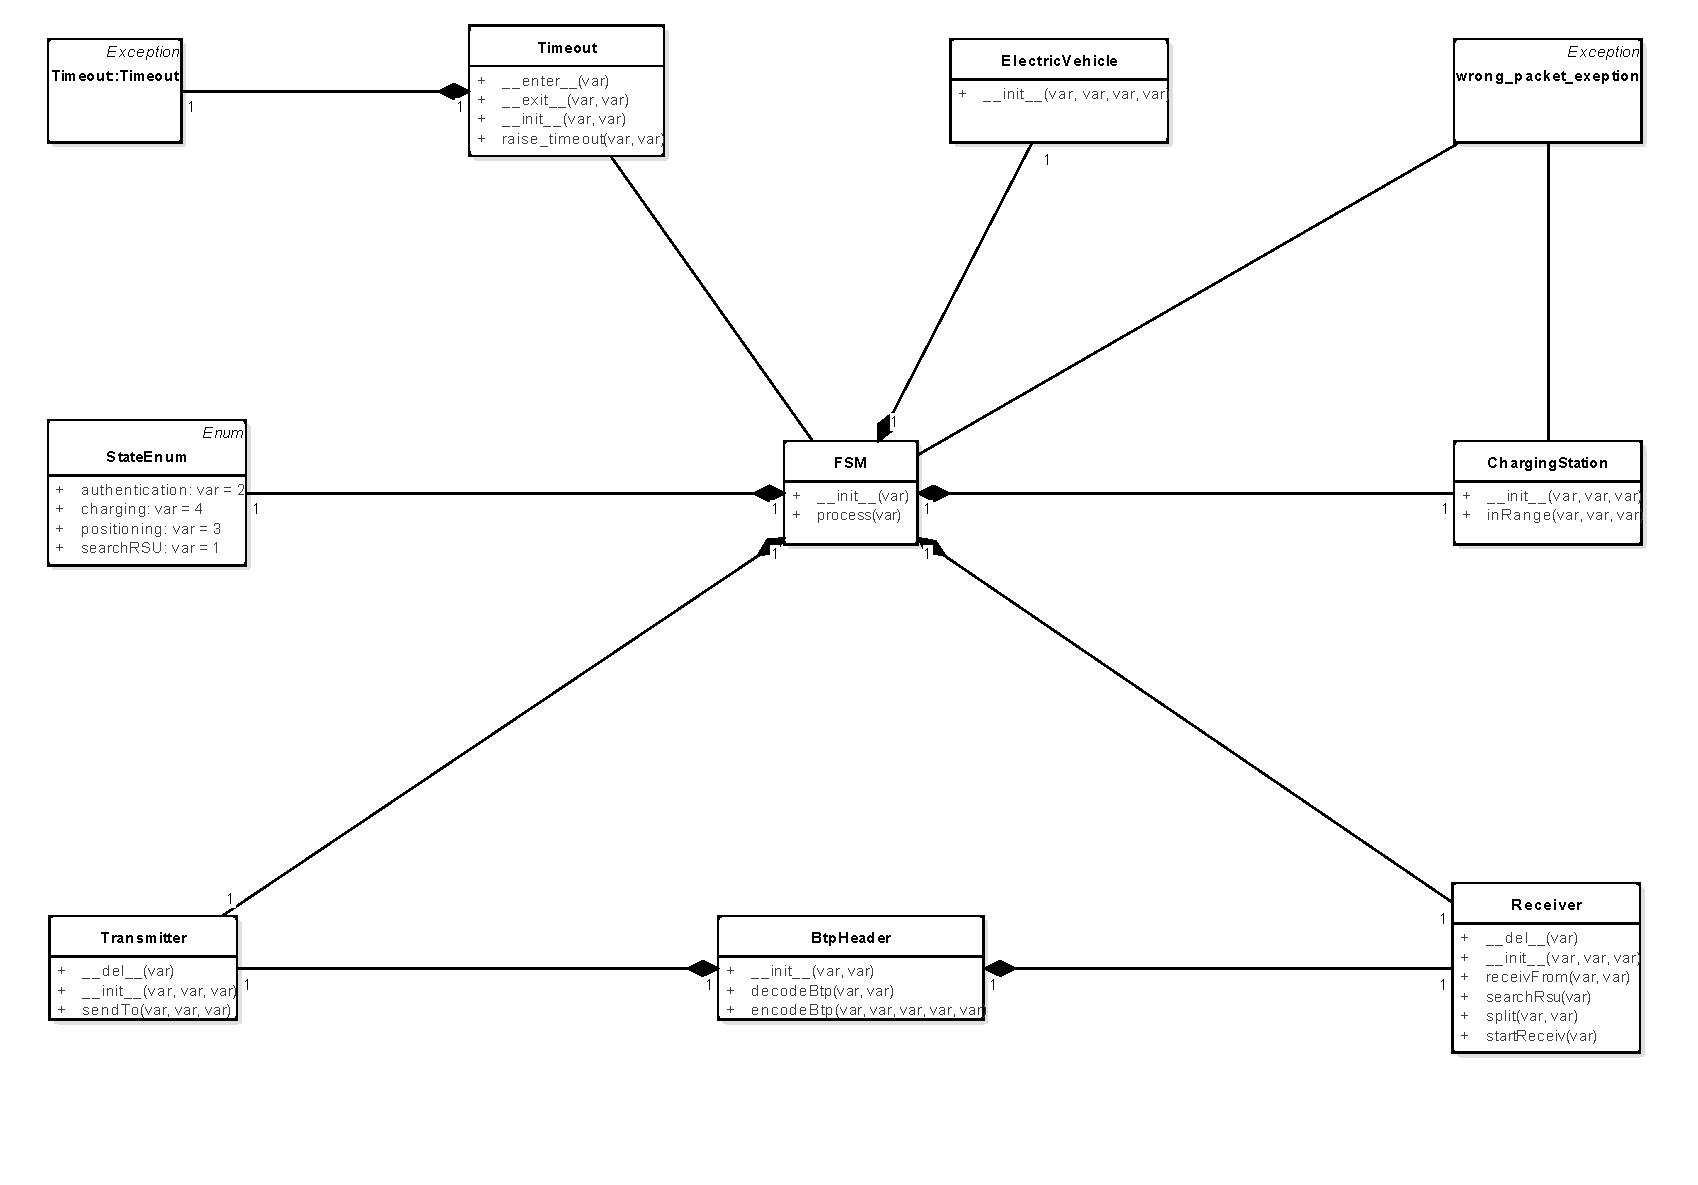
\includegraphics[width=1\textwidth]{images/class_OBU}
	\caption{Class Diagram of the Electric Vehicle}
	\label{fig:class_ev}
\end{figure}


\subsection{FSM}

The \textit{FSM} (finite state machine) is the class that controls the whole program. It is at the top level of the class hierarchy and the mediator between most classes. The constructor of the class initialises the whole system.

\subsection{BtpHeader}

On the Transmitter side, the \textit{BtpHeader} class encodes the payload to a BTP packet. There are two options to set up the BTP packets. 
\begin{itemize}
	\item \textbf{casttype} defines the cast type of the message: GeoUniCast or SingleHopBroadcast.
	\item If \textbf{secured} is set to 1, the payload will be encrypted.
\end{itemize}
On the receiver side, the \textit{BtpHeader} class decodes the received BTP Packets and decrypts the payload if needed.

\subsection{Receiver}

The ETSA application that runs on the MK5 (section \ref{sec:BTP_over_UDP}) sends all received BTP packets via UDP to the port 4400 of the Raspberry Pi. If the \textit{Receiver} class received a BTP message, the \textit{BtpHeader} class decodes the packet. The \textit{split} function of the \textit{Receiver} splits the payload to separate arguments and stores them in a list. Every argument is separated with a "$\setminus n$". This allows an easy access to the different arguments.

\begin{figure}[htb]
	\centering
	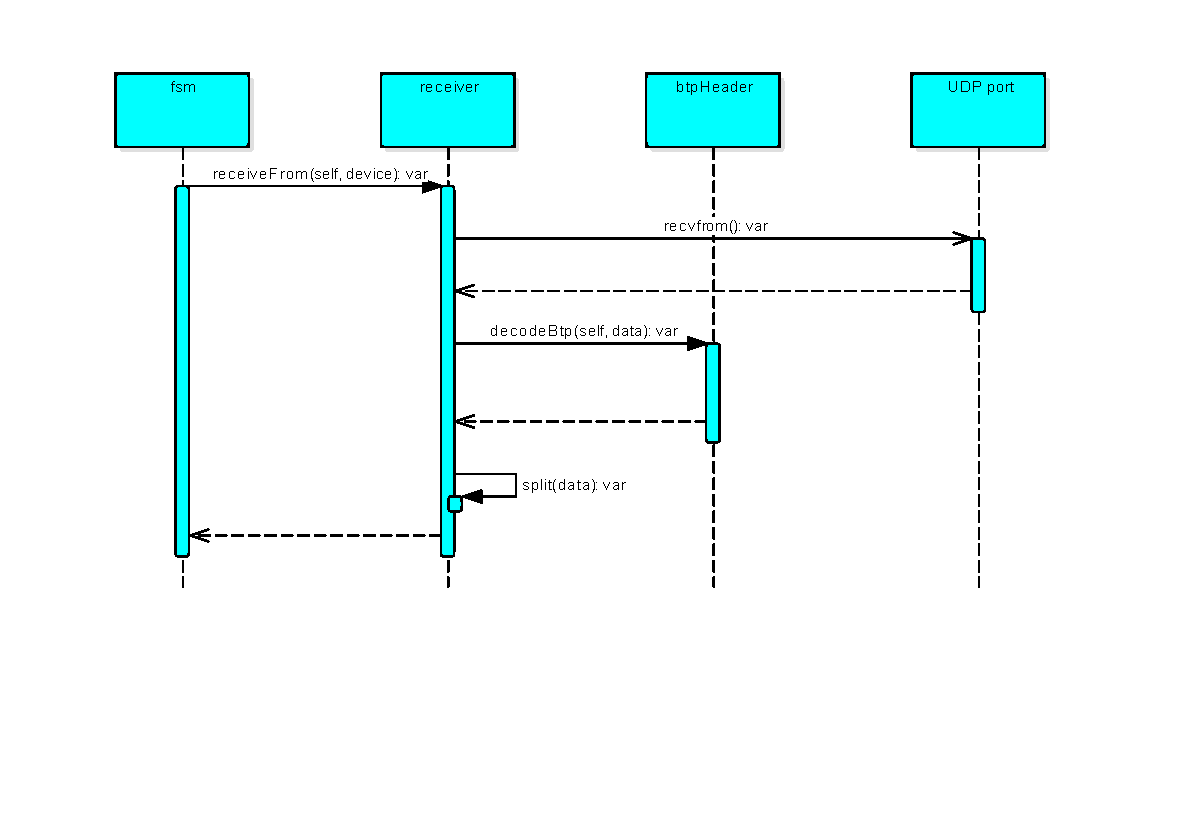
\includegraphics[width=1\textwidth]{images/Receive}
	\caption{Sequence Diagram of the Receiving Process}
	\label{fig:sequence_diagram_receive}
\end{figure}

\subsection{Transmitter}

To send a message to the charging station, a BTP packet must be created and send over UDP to MK5 OBU. The \textit{Transmitter} class takes care of this process. The message will be encoded to a BTP packet and sent to the UDP port of the MK5.

\begin{figure}[htb]
	\centering
	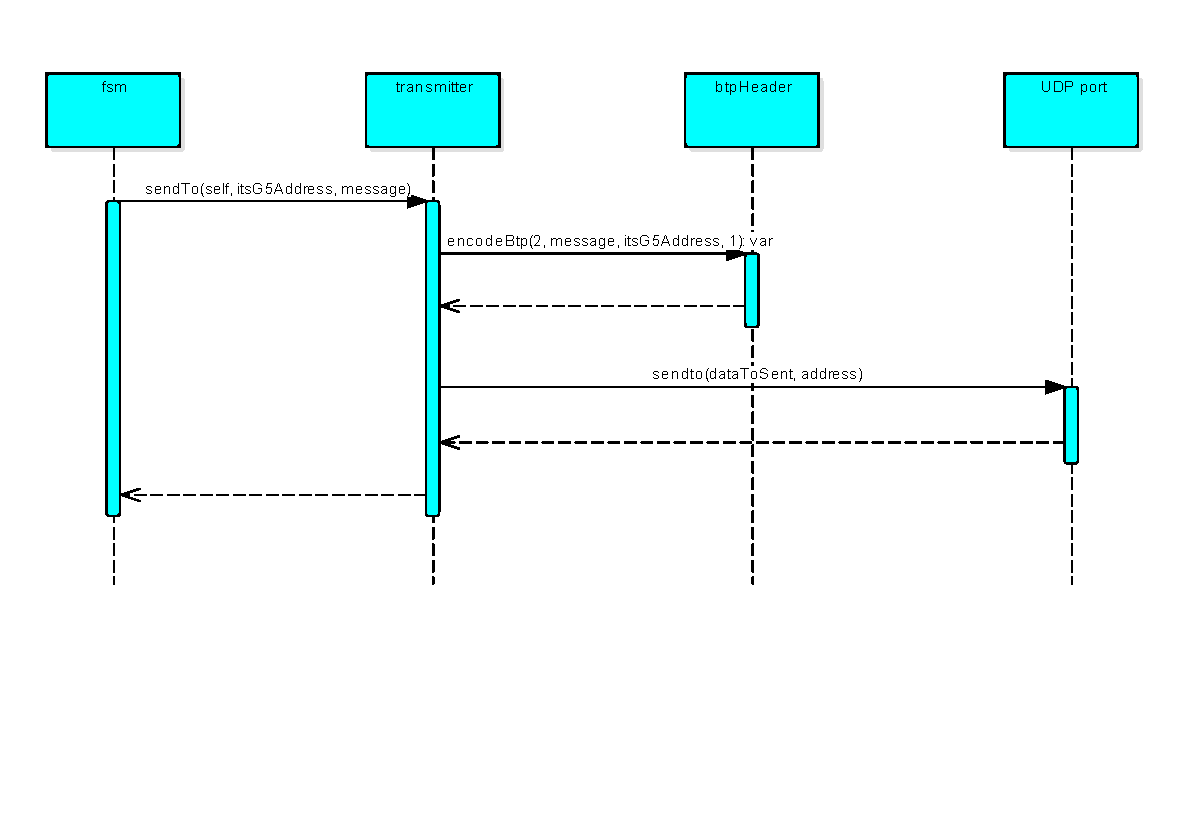
\includegraphics[width=1\textwidth]{images/transmit}
	\caption{Sequence Diagram of the Transmitting Process}
	\label{fig:sequence_diagram_transmit}
\end{figure}

\subsection{ChargingStation}

The \textit{ChargingStation} class stores information about the charging station. This information is provided to the electric vehicle at the beginning of the authentication process.

\subsection{ElectricVehicle}

At the initialization of the system, information about the electric vehicle is stored in the \textit{ElectricVehicle} class.

\newpage

\section{Charging Station}

The firmware of the charging station works similar to the one of the electric vehicle. The task of the charging station is to verify the identity of an electric vehicle and unlock the right charging device. The \textit{FSM}, \textit{ElectricVehicle}, \textit{ChargingStation}, \textit{Transmitter}, \textit{Receiver} and \textit{BtpHeader} are similar or the same as in the electric vehicle.

\begin{figure}[htb]
	\centering
	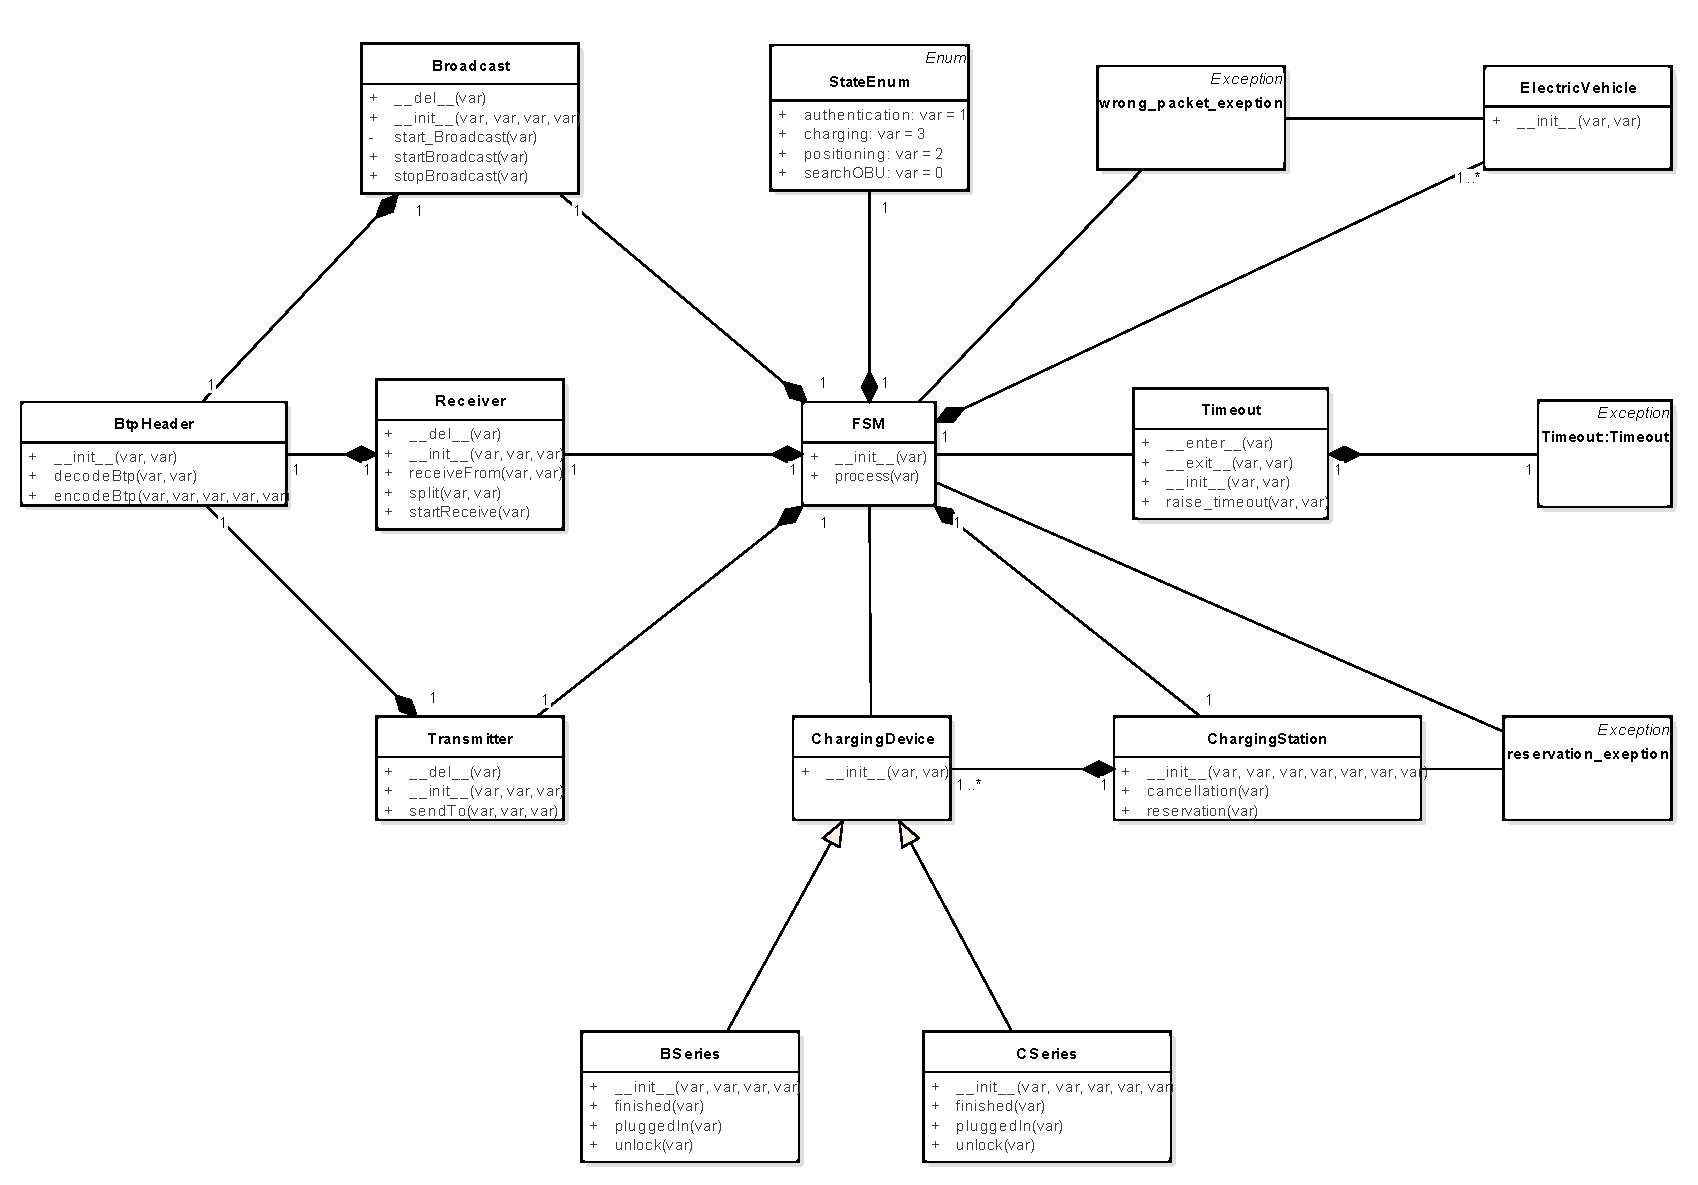
\includegraphics[width=1\textwidth]{images/class_RSU}
	\caption{Class Diagram of the Charging Station}
	\label{fig:class_cs}
\end{figure}

\subsection{Broadcast}

The \textit{Broadcast} class sends the status information periodical as broadcast message to all available ITS Stations (RSU and OBU). The \textit{Broadcast} class runs in a separate thread, so that an undisturbed process can be guaranteed. 

\subsection{ChargingDevice}

\textit{ChargingDevice} is the base class of \textit{BSeries} and \textit{Cseries} and controls the Charging Devices from Keba. The BSeries and CSeries are different types of charging devices as described in section \ref{sec:chargingDevices}. The BSeries is controlled with a relay switch. The CSeries is controlled with UDP. At the initialisation of the system the \textit{chargingDevices} are assigned to a parking lot. If the vehicle stands on the assigned parking lot, the charging device unlocks.   



